Eine flache Platte ist um eine feste Achse durch D drehbar, die senkrecht zur Platte steht. Im Punkt P, \rPO\ rechts von D, wirkt nacheinander eine Kraft von \FPO\ in vier verschiedenen Richtungen (siehe Abbildung, Kästchen \SI{10}{\cm}):
\begin{itemize}
 \item $\vec F_1$ in Richtung der Verbindungslinie von D nach P,
 \item $\vec F_2$ senkrecht zu DP nach oben,
 \item $\vec F_3$ unter \alO\ zu DP nach rechts oben,
 \item $\vec F_4$ unter \alO\ zu DP nach rechts unten.
\end{itemize}
\begin{center}
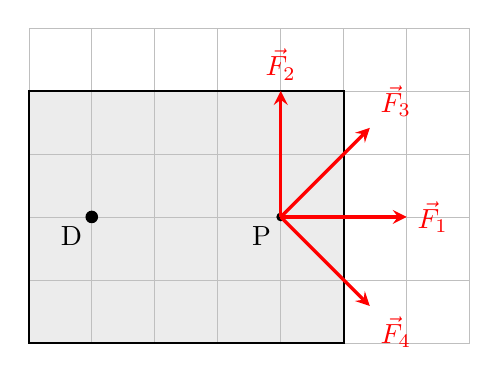
\begin{tikzpicture}[scale=0.8, >=stealth]
 \fill[gray!15] (-1,-2) rectangle (4,2);
 \draw[gray!50, very thin] (-1,-2) grid (6,3);
 \draw[thick] (-1,-2) rectangle (4,2);
 \fill (0,0) circle (0.1) node[below left] {D};
 \fill (3,0) circle (0.07) node[below left] {P};
 \draw[->, very thick, red] (3,0) -- (5,0) node[right] {$\vec F_1$};
 \draw[->, very thick, red] (3,0) -- (3,2) node[above] {$\vec F_2$};
 \draw[->, very thick, red] (3,0) -- (4.414,1.414) node[above right] {$\vec F_3$};
 \draw[->, very thick, red] (3,0) -- (4.414,-1.414) node[below right] {$\vec F_4$};
\end{tikzpicture}
\end{center}

\begin{abcliste}
\abc
Ordne die Drehmomente der vier Kräfte bezüglich D nach ihrem Betrag, das kleinste zuerst, ohne zu rechnen. Begründe mit den Wirkungslinien.

\abc
In welchem Drehsinn würde jede Kraft die Platte drehen?

\abc
Berechne die vier Drehmomente.
\end{abcliste}
